\begin{problem}{}{}{}{0.5 секунды}{64 Мб}
% Тетрис - Уровень 0

Коля перемещается в будущее и попадает в странную анфиладу комнат с витражами в синих меандрах.
Незнакомка в терракотовом платье даёт указание длинноволосому биороботу с механическим
голосом по имени Вертер завершить уборку и обесточить пульт. Так Вертер обнаруживает Колю,
задерживает его и проводит инвентаризацию. Вначале Вертер намеревается поместить Колю в музей,
но потом понимает, что это может дискредитировать Полину, в которую он безуспешно влюблён.
Он решает отправить мальчика обратно, открыв ему, что тот находится в 2084 году. Заинтригованный
Коля просит робота позволить ему хоть ненадолго взглянуть на будущее. Где если не в будущем можно
узнать достоверную информацию о прошлом? Так Коля и узнал, что 6 июня 1984 года была выпущена
культовая игра Тетрис.

{\bf {Тетрис}} "-- компьютерная игра, первоначально изобретённая и разработанная советским
программистом Алексеем Пажитновым. Игра была выпущена 6 июня 1984 года "-- в это время Пажитнов
работал в Вычислительном центре Академии наук СССР.

Тетрис представляет собой головоломку, построенную на использовании геометрических фигур
<<тетрамино>> "-- разновидности полимино, состоящих из четырёх квадратов.

\begin{wrapfigure}{r}{0.35\textwidth}
\vspace{-20pt}
  \begin{center}
    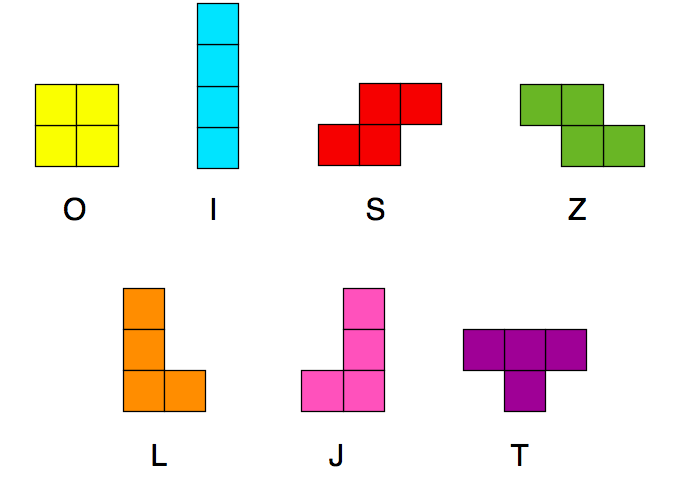
\includegraphics[width=0.35\textwidth,natwidth=267,natheight=200]{tetromino.png}
  \end{center}
  \vspace{-20pt}
  \vspace{1pt}
\end{wrapfigure}

Конечно же в 2084 году в компьютерные игры играют роботы, а не люди, поэтому и вместо
привычного клавиатурного управления игра была адаптирована для команд роботов.

К счастью, на нулевом уровне игры используются только тетрамино типа О (квадраты 2х2) и достаточно
сократить 100 строк чтобы перейти на следующий уровень.

{\bf {Правила игры}}

Фигурки тетрамино типа O падают сверху в прямоугольный стакан шириной 10 и высотой 20 клеток.
Как только тетрамино появляется робот-игрок может сдвинуть её по горизонтали, после чего
тетрамино летит вниз до тех пор, пока не наткнётся на другую фигурку либо на дно стакана. Если
при этом заполнился горизонтальный ряд из 10 клеток, он пропадает и всё, что выше него,
опускается на одну клетку.

Для того чтобы управлять тетрамино у роботов есть две команды: <<shift_left>> (сдвинуть влево) и
<<shift_right>> (сдвинуть вправо).

\InputFile
В каждой новой строке входного потока данных игра будет сообщать начальную позицию тетрамино
относительно левого края стакана (индексация с 1).

Игра сообщит число 0, когда вы проиграете или наберёте достаточное количество очков.

\OutputFile
На каждую строку ввода с указанием позиции очередного тетрамино программа должна сообщить набор
команд перемещения тетрамино, разделённых пробелом.

Если вы выведете некорректную команду, вы получите ответ PE; если вы проиграете раньше чем
сократите 10 строк, вы получите WA.

\Example

\begin{example}
\exmp{4

3

5

3

3

0
}{shift_left shift_left shift_left

shift_right shift_right shift_right shift_right shift_right shift_right

shift_left shift_left

shift_right shift_right

shift_right shift_right shift_right shift_right
}%
\end{example}

\Note
Задача не имеет однозначного ответа и оценивание будет проводиться по итогу нескольких игр, 
поэтому представленный вариант ответа "-- это лишь один из сотен возможных вариантов.

Первое тетрамино квадратной формы 2х2 появилось с отступом в 4 клетки от левого края и мы
решили сдвинуть его влево до упора; второе "-- появилось с отступом в 3 клетки и мы сдвинули
его до упора вправо; третье "-- мы приставили к первому, которое у левого края; четвёртое "--
пристроили к третьему; петое "-- заполнили оставшийся пробел между четвёртым и вторым. Таким
образом мы сократили сразу две строчки и наше поле снова чисто. Для краткости примера мы
остановили игру на этом шаге, получив от игры число 0.

Обратите внимание, игра не будет давать вам позицию следующего тетрамино пока вы не выведете
действия к текущему тетрамино!

\end{problem}

